%	proofeg.tex	(An example file for proof.sty)
%
%		Mar 6, 1997
%		Makoto Tatsuta
%
%	I hope you can learn how to use proof figure macros easily
%	by these examples.


\def\imp{\to}
\def\land{\mathbin\&}
% for LaTeX 2e naitive mode.
\documentclass[]{article}
\usepackage{proof}
\usepackage{tikz}
\usepackage{rotating}
\usepackage{enumitem}
\usetikzlibrary{trees}
\usetikzlibrary{positioning}

\tikzset{%
  zeroarrow/.style = {-stealth,dashed},
  onearrow/.style = {-stealth,solid},
  c/.style = {circle,draw,solid,minimum width=2em,
        minimum height=2em},
  r/.style = {rectangle,draw,solid,minimum width=2em,
        minimum height=2em}
}
\begin{document}

\section{Semantic Tableaux}
\textbf{a)} From the open leaves of the tableau we see that there are the following models that satisfy the formula $(p\rightarrow q) \rightarrow r$: $\{$
\begin{itemize}[noitemsep]
\item[] $\{(p\rightarrow F), (q, \rightarrow F), (r\rightarrow T)\},$
\item[] $\{(p\rightarrow F), (q, \rightarrow T), (r\rightarrow T)\},$
\item[] $\{(p\rightarrow T), (q, \rightarrow F), (r\rightarrow F)\},$
\item[] $\{(p\rightarrow T), (q, \rightarrow F), (r\rightarrow T)\},$
\item[] $\{(p\rightarrow T), (q, \rightarrow T), (r\rightarrow T)\}$
\end{itemize}$\}$. 
In the set of propositions $P = \{p, q, r\}$, the
formula $(\neg p \rightarrow r) \wedge (q \rightarrow r)$ has the same models $M((p\rightarrow q) \rightarrow r) = M((\neg p \rightarrow r) \wedge (q \rightarrow r))$. Therefore, we conclude that $(p\rightarrow q) \rightarrow r$ and $(\neg p \rightarrow r) \wedge (q \rightarrow r)$ are logically equivalent.

\begin{figure}[h]
\centering
\begin{tikzpicture}[level distance=1.5cm,
  level 1/.style={sibling distance=3cm},
  level 2/.style={sibling distance=1.5cm}]
  \node {$(p\rightarrow q) \rightarrow r$}
    child {node {$\neg (p \rightarrow q)$}
      child {node {$p, \neg q$}}
    }
    child {node {$r$}};
\end{tikzpicture}
\caption{Left-hand side} \label{fig:LHS}
\end{figure}

\begin{figure}[h]
\centering
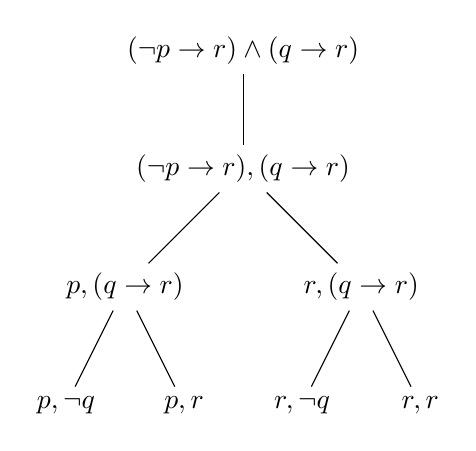
\begin{tikzpicture}[level distance=1.5cm,
  level 1/.style={sibling distance=3cm},
  level 3/.style={sibling distance=1.5cm}]
  \node {$(\neg p \rightarrow r) \wedge (q \rightarrow r)$}
    child {node {$(\neg p \rightarrow r),(q \rightarrow r)$}
      child {node {$p, (q\rightarrow r)$}
    	child {node {$p, \neg q$}}
   	    child {node {$p, r$}}
      }    	
      child {node {$r, (q\rightarrow r)$}
    	child {node {$r, \neg q$}}
   	    child {node {$r, r$}}      
      }
    };
\end{tikzpicture}
\caption{Right-hand side} \label{fig:RHS}
\end{figure}

\noindent \textbf{b)} To show that $(((p \rightarrow (q \wedge r)) \lor ((q \wedge r) \rightarrow p))\rightarrow p)$ is falsifiable, we must show that there exist models for the inverse, namely $\neg (((p \rightarrow (q \wedge r)) \lor ((q \wedge r) \rightarrow p))\rightarrow p)$. The semantic tableaux of the inverse can be found in Figure \ref{fig:both}. Two examples of interpretations which yield false are: $\{\{(p\rightarrow F), (q\rightarrow T), (r\rightarrow T)\},\{(p\rightarrow F),(q\rightarrow F),(r\rightarrow F)\}\}$


\begin{figure}[h]
\centering
\begin{tikzpicture}[level distance=1.5cm,
  level 1/.style={sibling distance=8cm},
  level 3/.style={sibling distance=5cm},
  level 4/.style={sibling distance=1.5cm}]
  \node {$\neg (((p \rightarrow (q \wedge r)) \lor ((q \wedge r) \rightarrow p))\rightarrow p)$}
    child {node {$(p \rightarrow (q \wedge r)) \lor ((q \wedge r) \rightarrow p), \neg p$}
      child {node {$p \rightarrow (q \wedge r), \neg p$}
    	child {node {$ \neg p, \neg p$}}
   	    child {node {$q \wedge r, \neg p$}
    	  child {node {$q,r, \neg p$}}
   	    }
      }    	
      child {node {$(q \wedge r) \rightarrow p, \neg p$}
    	child {node {$\neg (q \wedge r), \neg p$}
		  child {node {$\neg q, \neg p$}}
		  child {node {$\neg r, \neg p$}}
    	}
   	    child {node {$p, \neg p$}}      
      }
    };
\end{tikzpicture}
\caption{Semantic Tableaux for $\neg (((p \rightarrow (q \wedge r)) \lor ((q \wedge r) \rightarrow p))\rightarrow p)$} \label{fig:both}
\end{figure}

\section{Logical Equivalence}

\textbf{a)} \\
We prove by induction: \\
\textbf{basis} $n = 1$: $p_1 \equiv p_1$\\
\textbf{induction} $n > 1$ \\
Assumption: $\neg (p_1 \wedge ...\wedge p_{n-1}) \equiv \neg p_1 \vee ... \vee \neg p_{n-1}$\\
To prove: $\neg (p_1 \wedge ...\wedge p_{n-1} \wedge p_n) \equiv \neg p_1 \vee ... \vee \neg p_{n-1} \vee \neg p_n$\\
Deduction: \\
$\neg p1 \vee ... \vee \neg p_{n-1} \vee \neg p_n \\
\equiv (\neg p1 \vee ... \vee \neg p_{n-1}) \vee \neg p_n \\
\equiv \neg (p_1 \wedge ... \wedge p_{n-1}) \vee \neg p_n$   (substitute assumption) \\$
\equiv \neg ((p_1 \wedge ... \wedge p_{n-1}) \wedge p_n)$ (De Morgen's law) \\ $
\equiv \neg (p_1 \wedge ... \wedge p_{n-1} \wedge p_n)$ \\ \\

\noindent \textbf{Conclusion}: $\neg (p_n \wedge ... \wedge p_0) \equiv \neg p_n \vee ... \vee \neg p_1$

\noindent \textbf{b)}\\
We again prove by induction. \\
\textbf{Basis} $n = 1$: $ p_1 \rightarrow p_0 \equiv p_1 \rightarrow p_1$\\
\textbf{Induction} $n > 1$:\\
Assumption: $p_{n-1} \rightarrow (...\rightarrow(p_1 \rightarrow p_0)...) \equiv (p_{n-1} \wedge ... \wedge p_1)\rightarrow p_0$\\
To prove: $p_n\rightarrow (p_{n-1} \rightarrow (...\rightarrow(p_1 \rightarrow p_0)...)) \equiv (p_n \wedge p_{n-1} \wedge ... \wedge p_1)\rightarrow p_0$\\ 
Deduction:\\
$p_n\rightarrow (p_{n-1} \rightarrow (...\rightarrow(p_1 \rightarrow p_0)...)) \\
p_n \rightarrow ((p_{n-1} \wedge ... \wedge p_1) \rightarrow p_0)$ (substitute assumption) \\ $
\neg p_n \vee ((p_{n-1} \wedge ... \wedge p_1) \rightarrow p_0) \\
\neg p_n \vee \neg (p_{n-1} \wedge ... \wedge p_1) \vee p_0 \\
\neg (p_n \wedge (p_{n-1} \wedge ... \wedge p_1) \vee p_0$ (De Morgan's law) \\ $
\neg (p_n \wedge p_{n-1} \wedge ... \wedge p_1) \vee p_0 \\
(p_n \wedge p_{n-1} \wedge ... \wedge p_1) \rightarrow p_0$ \\ \\

\noindent \textbf{Conclusion}: $p_n\rightarrow (p_{n-1} \rightarrow (...\rightarrow(p_1 \rightarrow p_0)...)) \equiv (p_n \wedge p_{n-1} \wedge ... \wedge p_1)\rightarrow p_0$\\ \\

\section{Gentzen}
$$
\infer[(L_\leftrightarrow)]{\Gamma, \phi \leftrightarrow \psi\vdash\Delta}{\Gamma, \phi \rightarrow \psi, \psi \rightarrow \phi\vdash\Delta}
$$

$$
\infer[(R_\leftrightarrow)]{\Gamma\vdash\Delta, \phi \leftrightarrow \psi}{
\Gamma \vdash \Delta, \phi \rightarrow \psi
&
\Gamma \vdash \Delta, \psi \rightarrow \phi
}
$$
\begin{sidewaysfigure}
    \centering
\begingroup\makeatletter\def\f@size{5}\check@mathfonts
$$
\infer[R_\rightarrow]{\vdash ((p \leftrightarrow q) \wedge (q \leftrightarrow r)) \rightarrow (r \leftrightarrow p)}{
	\infer[L_\wedge]{((p \leftrightarrow q) \wedge (q \leftrightarrow r)) \vdash (r \leftrightarrow p)}{
		\infer[L_\leftrightarrow]{(p \leftrightarrow q), (q \leftrightarrow r) \vdash (r \leftrightarrow p)}{	
			\infer[L_\leftrightarrow]{(p \rightarrow q),(q \rightarrow p), (q \leftrightarrow r) \vdash (r \leftrightarrow p)}{		
				\infer[R_\leftrightarrow]{(p \rightarrow q),(q \rightarrow p), (q \rightarrow r),(r \rightarrow q) \vdash (r \leftrightarrow p)}{	
					\infer[R_\rightarrow]{(p \rightarrow q),(q \rightarrow p), (q \rightarrow r),(r \rightarrow q) \vdash (r \rightarrow p)}{
						\infer[L_\rightarrow]{r,(p \rightarrow q),(q \rightarrow p), (q \rightarrow r),(r \rightarrow q) \vdash p}{
							r,(p \rightarrow q),(q \rightarrow p), (q \rightarrow r) \vdash p,r 
							&
							\infer[L_\rightarrow]{r,q,(p \rightarrow q),(q \rightarrow p), (q \rightarrow r) \vdash p}{
								r,q,(p \rightarrow q), (q \rightarrow r) \vdash p,q
								&
								r,q,p,(p \rightarrow q), (q \rightarrow r) \vdash p 
							} 
						}	
					}	
					&
					\infer[R_\rightarrow]{(p \rightarrow q),(q \rightarrow p), (q \rightarrow r),(r \rightarrow q) \vdash (p \rightarrow r)}{	
						\infer[L_\rightarrow]{p,(p \rightarrow q),(q \rightarrow p), (q \rightarrow r),(r \rightarrow q) \vdash r}{	
							p,(q \rightarrow p), (q \rightarrow r),(r \rightarrow q) \vdash r,p
							&
							\infer[L_\rightarrow]{p,q,(q \rightarrow p), (q \rightarrow r),(r \rightarrow q) \vdash r}{	
								p,q,(q \rightarrow p),(r \rightarrow q) \vdash r,q
								&
								p,q,r,(q \rightarrow p),(r \rightarrow q) \vdash r 
							}	 
						}	
					}			
				}			
			}				
		}
	}
}
$$\endgroup
	\caption{Proof for $\vdash ((p \leftrightarrow q) \wedge (q \leftrightarrow r)) \rightarrow (r \leftrightarrow p)$ in $G$}
    \label{fig:awesome_image}
\end{sidewaysfigure}

\section{Hilbert}
In order to solve the theorem in H we first transform the formula eliminating all operators except for $\neg$ and $\rightarrow$. \\ 
$$(p \rightarrow (q \rightarrow r)) \rightarrow ((p \wedge q) \rightarrow r)
\equiv p \rightarrow (q \rightarrow r )) \rightarrow (\neg (p \rightarrow \neg q) \rightarrow r)
$$

\noindent To shorten the eventual proof we first prove that $\vdash \neg (p \rightarrow q) \rightarrow p$ and $\vdash (p \rightarrow q) \rightarrow q$. \\ \\
\noindent Theorem 4.1:
$$
\infer
	{\vdash \neg(p \rightarrow \neg q) \rightarrow p}
	{\infer
		{\neg (p \rightarrow \neg q) \vdash p}
		{\infer
			{p \wedge q \vdash p}
			{p, q \vdash p}
		}
	}
$$\\

\noindent Theorem 4.2:
$$
\infer
	{\vdash \neg(p \rightarrow \neg q) \rightarrow q}
	{\infer
		{\neg (p \rightarrow \neg q) \vdash q}
		{\infer
			{p \wedge q \vdash q}
			{p, q \vdash q}
		}
	}
$$\\

\noindent The proof of $(p \rightarrow (q \rightarrow r)) \rightarrow (\neg (p \rightarrow \neg q) \rightarrow r)$ is listed in figure \ref{fig:proofH}. \\

\begin{sidewaysfigure}
    \centering
\begingroup\makeatletter\def\f@size{5}\check@mathfonts
$$
\infer[DR]{\vdash (p \rightarrow (q \rightarrow r)) \rightarrow (\neg (p \rightarrow \neg q) \rightarrow r)}{
	\infer[DR] {p \rightarrow (q \rightarrow r) \vdash \neg (p \rightarrow \neg q) \rightarrow r}{
		\infer[MP]{p \rightarrow (q \rightarrow r), \neg (p \rightarrow \neg q) \vdash  r}{
			\infer[MP]{p \rightarrow (q \rightarrow r), \neg (p \rightarrow \neg q) \vdash q}{
				p \rightarrow (q \rightarrow r), \neg (p \rightarrow \neg q) \vdash \neg (p \rightarrow \neg q)
				&
				\infer{\Gamma \vdash \neg (p \rightarrow \neg q) \rightarrow q}{
					Theorem 4.2
				}
			}
			&
			\infer[MP]{p \rightarrow (q \rightarrow r), \neg (p \rightarrow \neg q) \vdash q \rightarrow r}{
				\infer[MP]{p \rightarrow (q \rightarrow r), \neg (p \rightarrow \neg q) \vdash p}{
					p \rightarrow (q \rightarrow r), \neg (p \rightarrow \neg q) \vdash \neg (p \rightarrow \neg q)
					&
					\infer{\Gamma \vdash \neg (p \rightarrow \neg q) \rightarrow p}{
						Theorem 4.1
					}
				}
				&
				p \rightarrow (q \rightarrow r), \neg (p \rightarrow \neg q) \vdash p \rightarrow (q \rightarrow r)
			}
		}
	}
}
$$\endgroup
	\caption{Proof for $(p \rightarrow (q \rightarrow r)) \rightarrow (\neg (p \rightarrow \neg q) \rightarrow r))$ in $H$}
    \label{fig:proofH}
\end{sidewaysfigure}

\noindent Conclusion: $\vdash (p \rightarrow (q \rightarrow r) \rightarrow ((p \wedge q) \rightarrow r)$.

\section{Clausal From}
\section{BDDs}
When we use the Apply algorithm on the sub-BDD for subformula $p \wedge q$, combined with the sub-BDD for the formula $r$ using the $\rightarrow$ operator, we get the BDD for $(p \wedge q)\rightarrow r$:

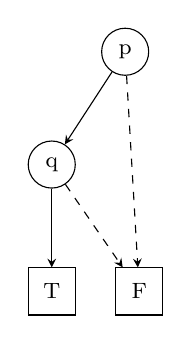
\begin{tikzpicture}[node distance=1cm and 0.5cm]\footnotesize
   \node[c] (p) {p};
   \node[c] (q) [below left=of p] {q};
   \node[r] (final-one) [below =of q] {T};
   \node[r] (final-zero) [right=of final-one] {F};
   \draw[onearrow] (p) -- (q);
   \draw[onearrow] (q) -- (final-one);
   \draw[zeroarrow] (p) -- (final-zero);
   \draw[zeroarrow] (q) -- (final-zero);
\end{tikzpicture}
\indent $\rightarrow$ \indent 
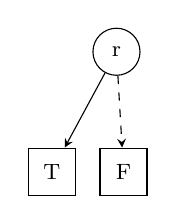
\begin{tikzpicture}[node distance=1cm and 0.3cm]\footnotesize
   \node[c] (r) {r};
   \node[r] (final-one) [below left=of r] {T};
   \node[r] (final-zero) [right=of final-one] {F};
   \draw[onearrow] (r) -- (final-one);
   \draw[zeroarrow] (r) -- (final-zero);
\end{tikzpicture}
\indent $=$ \indent 
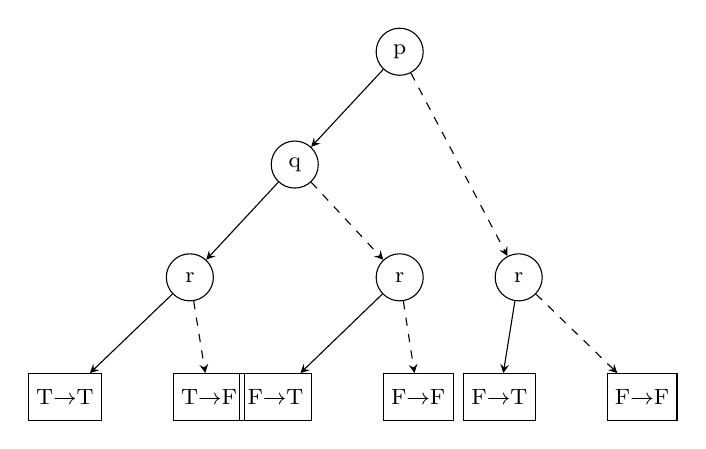
\begin{tikzpicture}[node distance=1cm and 0.9cm]\footnotesize
   \node[c] (p) {p};
   \node[c] (q) [below left=of p] {q};
   \node[c] (r1) [below left=of q] {r};
   \node[r] (final-one1) [below left=of r1] {T$\rightarrow$T};
   \node[r] (final-zero1) [right=of final-one1] {T$\rightarrow$F};
   
   \node[c] (r2) [below right=of q] {r};
   \node[r] (final-one2) [below left=of r2] {F$\rightarrow$T};
   \node[r] (final-zero2) [right=of final-one2] {F$\rightarrow$F};

   \node[c] (r3) [right=of r2] {r};
   \node[r] (final-zero3) [below right=of r3] {F$\rightarrow$F};
   \node[r] (final-one3) [left=of final-zero3] {F$\rightarrow$T};

   \draw[onearrow] (p) -- (q);
   \draw[onearrow] (q) -- (r1);
   \draw[onearrow] (r1) -- (final-one1);
   \draw[onearrow] (r2) -- (final-one2);
   \draw[onearrow] (r3) -- (final-one3);
   \draw[zeroarrow] (p) -- (r3);
   \draw[zeroarrow] (q) -- (r2);
   \draw[zeroarrow] (r1) -- (final-zero1);
   \draw[zeroarrow] (r2) -- (final-zero2);
   \draw[zeroarrow] (r3) -- (final-zero3);
\end{tikzpicture}
\\
\\
When we apply the Reduce algorithm on this result we get:
\\
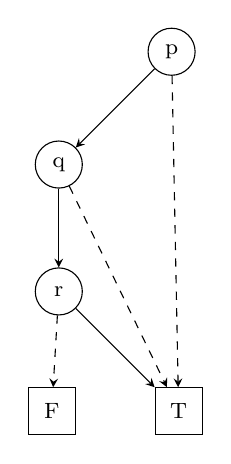
\begin{tikzpicture}[node distance=1cm and 1cm]\footnotesize
   \node[c] (p) {p};
   \node[c] (q) [below left=of p] {q};

   \node[c] (r) [below=of q] {r};
   \node[r] (final-one) [below right=of r] {T};
   \node[r] (final-zero) [left=of final-one] {F};

   \draw[onearrow] (p) -- (q);
   \draw[onearrow] (q) -- (r);
   \draw[onearrow] (r) -- (final-one);

   \draw[zeroarrow] (p) --(final-one);
   \draw[zeroarrow] (r) -- (final-zero);
   \draw[zeroarrow] (q) -- (final-one);
\end{tikzpicture}\\
\\
We will now use the Apply algorithm on the sub-BDD for subformula $p$, combined with the sub-BDD for the formula $q \rightarrow r$ using the $\rightarrow$ operator, to get the BDD for $p \rightarrow (q\rightarrow r)$:
\\
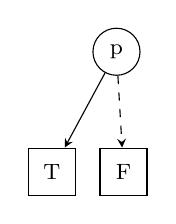
\begin{tikzpicture}[node distance=1cm and 0.3cm]\footnotesize
   \node[c] (p) {p};
   \node[r] (final-one) [below left=of p] {T};
   \node[r] (final-zero) [right=of final-one] {F};
   \draw[onearrow] (p) -- (final-one);
   \draw[zeroarrow] (p) -- (final-zero);
\end{tikzpicture}
\indent $\rightarrow$ \indent 
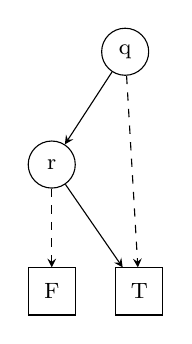
\begin{tikzpicture}[node distance=1cm and 0.5cm]\footnotesize
   \node[c] (q) {q};
   \node[c] (r) [below left=of q] {r};
   \node[r] (final-zero) [below =of r] {F};
   \node[r] (final-one) [right=of final-zero] {T};

   \draw[onearrow] (q) -- (r);
   \draw[onearrow] (r) -- (final-one);

   \draw[zeroarrow] (q) -- (final-one);
   \draw[zeroarrow] (r) -- (final-zero);
\end{tikzpicture}
\indent $=$ \indent 
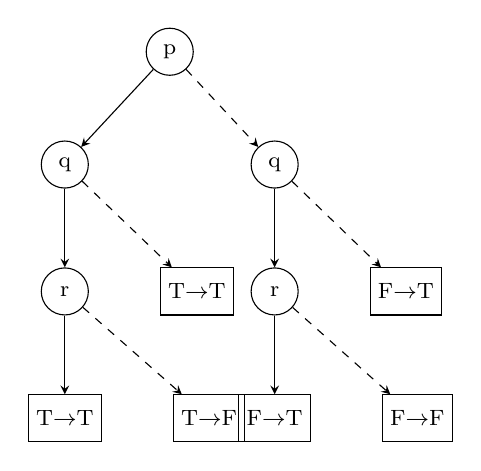
\begin{tikzpicture}[node distance=1cm and 0.9cm]\footnotesize
   \node[c] (p) {p};
   \node[c] (q1) [below left=of p] {q};
   \node[c] (q2) [below right=of p] {q};
   \node[c] (r1) [below =of q1] {r};
   \node[c] (r2) [below =of q2] {r};
   \node[r] (final-one1) [below=of r1] {T$\rightarrow$T};
   \node[r] (final-zero1) [right=of final-one1] {T$\rightarrow$F};
  
   \node[r] (final-one2) [below=of r2] {F$\rightarrow$T};
   \node[r] (final-zero2) [right=of final-one2] {F$\rightarrow$F};

   \node[r] (final-zero3) [right=of r1] {T$\rightarrow$T};
   \node[r] (final-zero4) [right=of r2] {F$\rightarrow$T};

   \draw[onearrow] (p) -- (q1);
   \draw[onearrow] (q1) -- (r1);
   \draw[onearrow] (q2) -- (r2);
   \draw[onearrow] (r1) -- (final-one1);
   \draw[onearrow] (r2) -- (final-one2);

   \draw[zeroarrow] (p) -- (q2);
   \draw[zeroarrow] (q1) -- (final-zero3);
   \draw[zeroarrow] (r1) -- (final-zero1);
   \draw[zeroarrow] (q2) -- (final-zero4);
   \draw[zeroarrow] (r2) -- (final-zero2);
\end{tikzpicture}
\\
\\
When we apply the Reduce algorithm on this result we (again) get:\\
\\
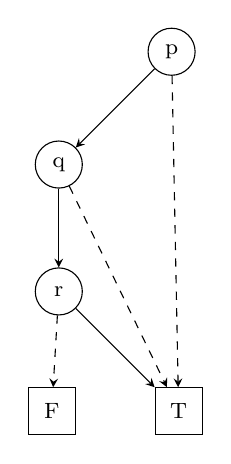
\begin{tikzpicture}[node distance=1cm and 1cm]\footnotesize
   \node[c] (p) {p};
   \node[c] (q) [below left=of p] {q};

   \node[c] (r) [below=of q] {r};
   \node[r] (final-one) [below right=of r] {T};
   \node[r] (final-zero) [left=of final-one] {F};

   \draw[onearrow] (p) -- (q);
   \draw[onearrow] (q) -- (r);
   \draw[onearrow] (r) -- (final-one);

   \draw[zeroarrow] (p) --(final-one);
   \draw[zeroarrow] (r) -- (final-zero);
   \draw[zeroarrow] (q) -- (final-one);
\end{tikzpicture}\\
\\
If we now use the Apply algorithm using the previously obtained sub-BDDs and the $\rightarrow$ operator, we get the BDD for $(p\rightarrow(q\rightarrow r))\rightarrow((p\wedge q)\rightarrow r)$:\\
\\
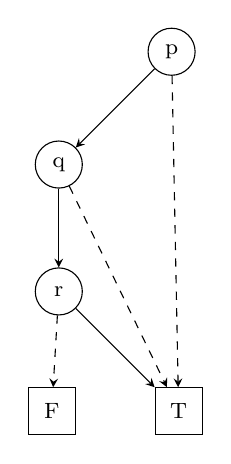
\begin{tikzpicture}[node distance=1cm and 1cm]\footnotesize
   \node[c] (p) {p};
   \node[c] (q) [below left=of p] {q};

   \node[c] (r) [below=of q] {r};
   \node[r] (final-one) [below right=of r] {T};
   \node[r] (final-zero) [left=of final-one] {F};

   \draw[onearrow] (p) -- (q);
   \draw[onearrow] (q) -- (r);
   \draw[onearrow] (r) -- (final-one);

   \draw[zeroarrow] (p) --(final-one);
   \draw[zeroarrow] (r) -- (final-zero);
   \draw[zeroarrow] (q) -- (final-one);
\end{tikzpicture}
\indent $\rightarrow$ \indent 
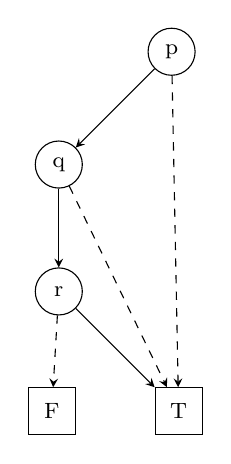
\begin{tikzpicture}[node distance=1cm and 1cm]\footnotesize
   \node[c] (p) {p};
   \node[c] (q) [below left=of p] {q};

   \node[c] (r) [below=of q] {r};
   \node[r] (final-one) [below right=of r] {T};
   \node[r] (final-zero) [left=of final-one] {F};

   \draw[onearrow] (p) -- (q);
   \draw[onearrow] (q) -- (r);
   \draw[onearrow] (r) -- (final-one);

   \draw[zeroarrow] (p) --(final-one);
   \draw[zeroarrow] (r) -- (final-zero);
   \draw[zeroarrow] (q) -- (final-one);
\end{tikzpicture}
\indent $=$ \indent 
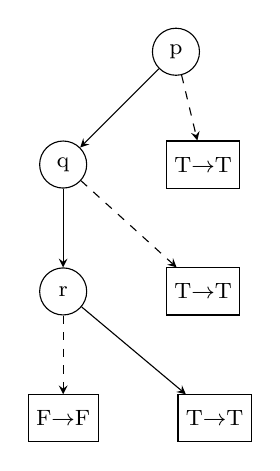
\begin{tikzpicture}[node distance=1cm and 1cm]\footnotesize
   \node[c] (p) {p};
   \node[c] (q) [below left=of p] {q};

   \node[c] (r) [below=of q] {r};
   \node[r] (final-zero1) [below=of r] {F$\rightarrow$F};
   \node[r] (final-one) [right=of final-zero1] {T$\rightarrow$T};
   \node[r] (final-zero2) [right=of r] {T$\rightarrow$T};
   \node[r] (final-zero3) [right=of q] {T$\rightarrow$T};

   \draw[onearrow] (p) -- (q);
   \draw[onearrow] (q) -- (r);
   \draw[onearrow] (r) -- (final-one);

   \draw[zeroarrow] (p) --(final-zero3);
   \draw[zeroarrow] (r) -- (final-zero1);
   \draw[zeroarrow] (q) -- (final-zero2);
\end{tikzpicture}\\
\\
When we apply the Reduce algorithm on this result we get 
\begin{tikzpicture}\footnotesize\node[r] (T) {T};\end{tikzpicture} which means that $\models (p\rightarrow(q\rightarrow r))\rightarrow((p\wedge q)\rightarrow r)$ holds, since it yields $True$ for all values of $p$, $q$ and $r$.
\section{...}
\section{The Lady, or the Tiger?}
\end{document}
